\documentclass[12pt]{zettel}

\usepackage{multicol}

%\renewcommand{\gregor}{\put(10.0,-3.5){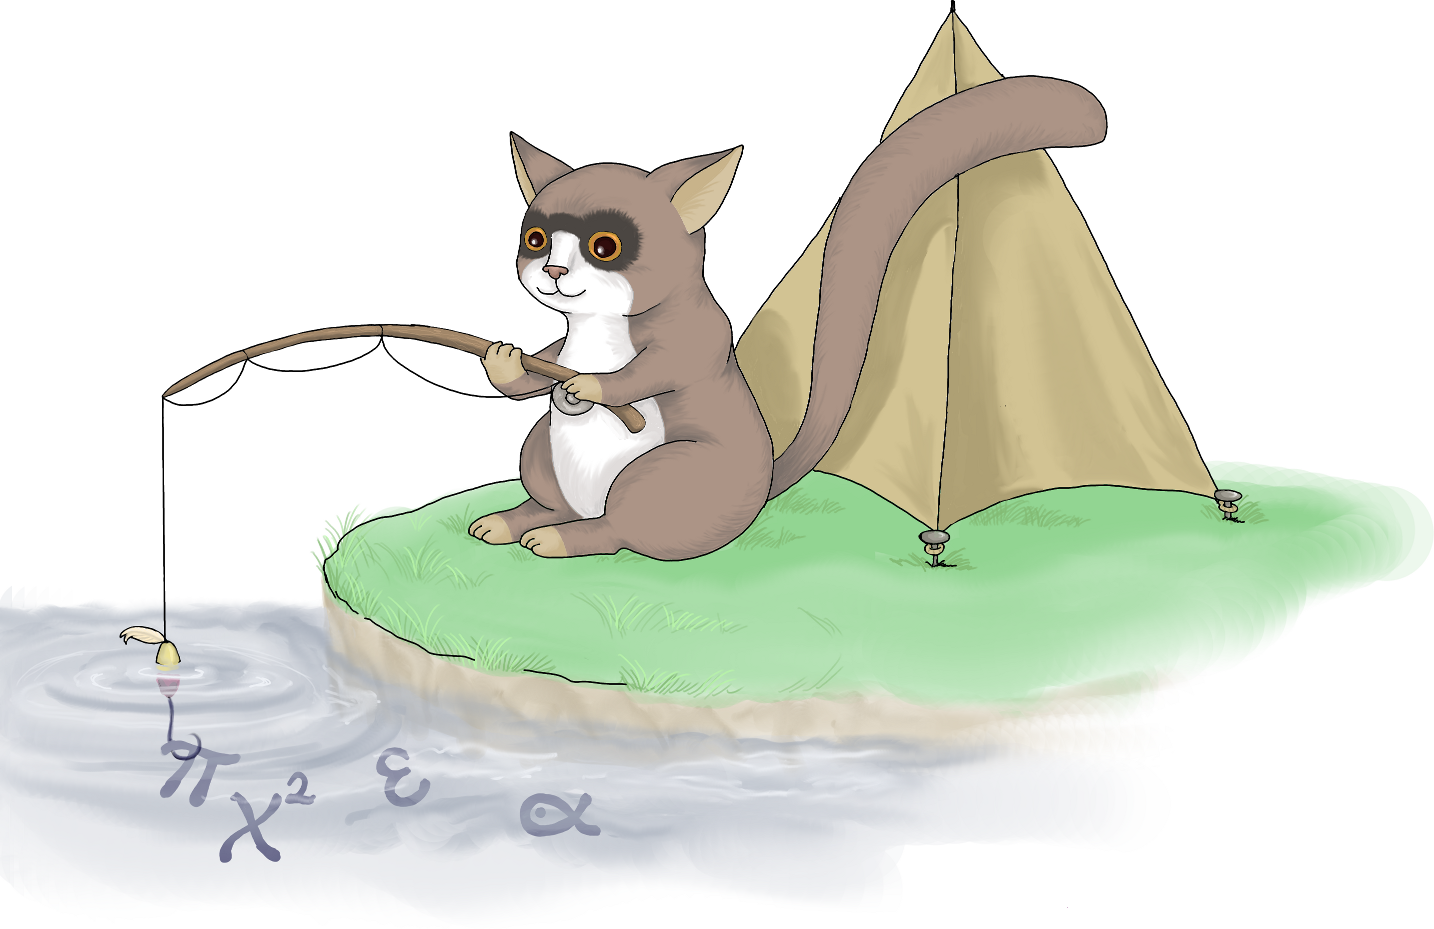
\includegraphics[scale=0.18]{campgregor}}}

\usepackage{framed}
\definecolor{shadecolor}{rgb}{.97,.97,.97}

\geometry{tmargin=1.5cm,bmargin=1.5cm,lmargin=2.5cm,rmargin=2.5cm}

\renewcommand{\gregor}{\put(9.2,-3.5){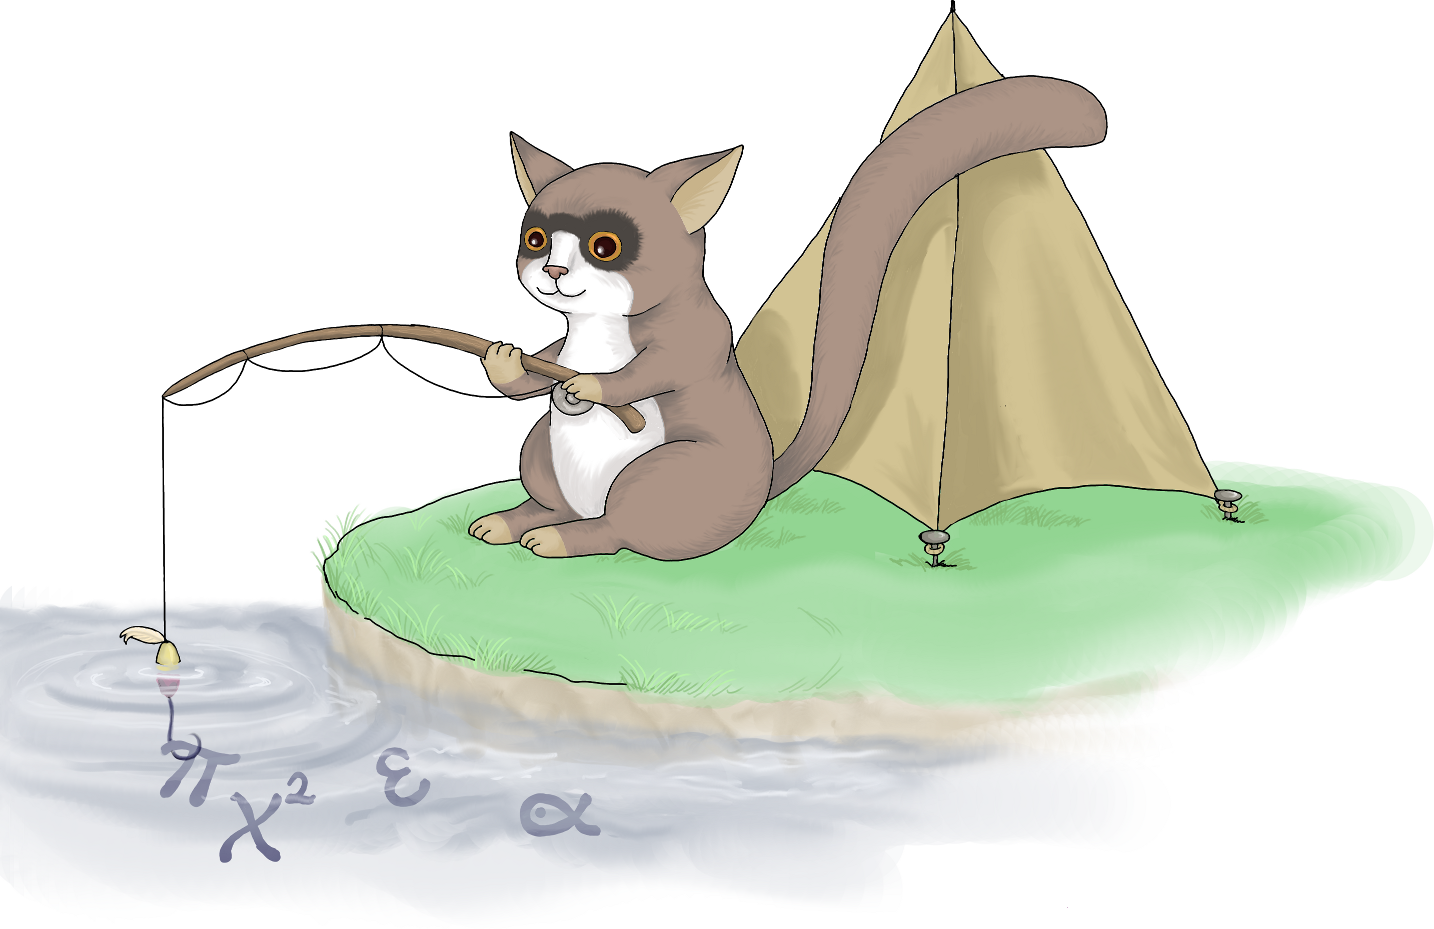
\includegraphics[scale=0.18]{campgregor}}}
\begin{document}

\renewcommand{\betreff}{Mathecamp des Matheschülerzirkels Augsburg vom 16. bis
20. August}

\makeletterhead{}
\vspace{-2em}

Liebe Schülerinnen und Schüler, liebe Eltern,

wir freuen uns, dass ihr mit uns vom 16. bis 20. August aufs Mathecamp kommt.
Mit diesem Schreiben informieren wir euch über ein paar Details.
\textbf{XXX: Diese Sätze sind super schlecht.}

\begin{shaded}
\textbf{Anreise per Bus.} Falls ihr auf der Anmeldung angegeben habt, dass ihr mit dem
Mathezirkelbus nach Violau fahren möchtet, kommt bitte am 16. August um
9:30 Uhr zum Messeparkplatz bei der Uni Augsburg: Universitätsstr. 16, 86159
Augsburg. Karte: \url{https://goo.gl/maps/h4lBY}

\textbf{Individuelle Anreise.} Falls ihr nicht mit uns nach Violau fahrt, kommt
zwischen 10:00 Uhr und 11:00 Uhr direkt zum Bruder-Klaus-Heim:
St. Michael Straße 15, 86450 Violau-Altenmünster
\end{shaded}

\begin{shaded}
\textbf{Kontakt.}
\begin{tabbing}
  während des Camps: \= \kill
  vor dem Camp: \> Büro: 0821/598-5601, 0821/598-5805 \\
  während des Camps: \> Handy: 0160/1111111111, 0160/2222222222, 0160/33333333333 \\
  \> Festnetz des Bruder-Klaus-Heims: 08295/1097 \\
  \> Fax: 08295/499
\end{tabbing}
\end{shaded}

\begin{shaded}
\textbf{Packliste.}

\begin{multicols}{2}
\begin{itemize}
\item \textbf{Krankenkassenkarte}
\item \textbf{ggf. Medikamente}
\item \textbf{Kleidung} (auch für Freizeit/Sport)
\item \textbf{Kulturbeutel}
\item \textbf{Handtuch}
\item \textbf{Bettwäsche} (oder 5 EUR)
\item Mäppchen mit Stiften und Geodreieck
\item Block zum Mitschreiben
\item Hallenschuhe
\item Taschenlampe
\item Handy
\item ggf. Schwimmsachen
\item ggf. Bücher
\item ggf. (Brett-)Spiele (falls ihr ein Lieblingsspiel habt, dass ihr mit anderen
spielen wollt)
\item ggf. Musikinstrument
\item Süßigkeiten/Knabberzeugs (aber nicht "`zu viele Kekse"' \textbf{XXX: Was
bedeutet das?})
\item Geld für Getränke
\item Auch ohne viele elektronische Geräte werdet ihr nicht vor Langeweile
sterben. Alkohol, Messer u.\,Ä. darf nicht mitgebracht werden.
\end{itemize}
\end{multicols}
\end{shaded}

\end{document}
